\documentclass[12pt, letterpaper]{article}
\usepackage[letterpaper,margin=1in]{geometry}
\usepackage[utf8]{inputenc} % allow utf-8 input
\usepackage[T1]{fontenc}    % use 8-bit T1 fonts
\usepackage{hyperref}       % hyperlinks
\usepackage{url}            % simple URL typesetting
\usepackage{booktabs}       % professional-quality tables
\usepackage{amsfonts}       % blackboard math symbols
\usepackage{nicefrac}       % compact symbols for 1/2, etc.
\usepackage{lipsum}
\usepackage{comment}
\usepackage[ruled,vlined,boxed]{algorithm2e}
\usepackage{graphicx}
\usepackage{natbib}
\bibliographystyle{apalike}
\usepackage{amsmath}
\DeclareMathOperator*{\argmax}{argmax} 
\linespread{1.0}

\title{Multi-Armed Bandits with Variance Considerations}
\date{}
\author{}
\begin{document}
\maketitle

\begin{abstract}
Multi-armed bandits (MAB) are sequential experimentation procedures that use a combination of exploration and exploitation techniques in order to reduce the total number of allocations to interventions with sub-optimal outcomes. MAB's are very effective in reducing the regret of the experimentation process compared to A/B testing especially in the presence of multiple policy levers. However, unlike A/B testing, MAB's may fail to accurately estimate the mean and variance of outcome distributions of interventions. In many marketing, clinical trial and public policy settings, mean and variance estimation of all interventions is as important as that of the best intervention, e.g., clinicians prefer lower variance treatments compared to higher ones even if the latter is slightly more effective. In this paper, we propose a new MAB algorithm that does variance based dynamic allocation. We show that the new algorithm has regret comparable to best MAB algorithms while having the variance estimation properties of A/B testing. 
\end{abstract}

% keywords can be removed
{Keywords: Multi-armed bandit, A/B testing, variance estimation}

\section*{Introduction}
A/B testing is an experimentation strategy used to infer the effectiveness of an intervention compared to a baseline (control). A/B testing is used in many scientific fields like Agriculture, Medicine, Social sciences and online experimentation. Due to the proliferation of internet technologies, A/B testing is widely used on internet platforms like Amazon, Microsoft, Google, etc \citep{kohavi2009controlled}. It is used in a variety of tasks, e.g., to test various design features of a website, test various marketing campaigns, etc. For a given tolerance of Type 1 and Type 2 errors, A/B testing is very effective in statistically rejecting a null hypothesis (i.e. the intervention has no additional benefit compared to the baseline). During an A/B test, units are allocated randomly to the baseline condition (control group) and the interventions (treatment groups). If the mean of the treatment outcomes is statistically different compared to the mean of control outcomes, we consider treatment to be effective.  Typically, multiple variants of a feature/ad/promotion are tested during the exploration phase of an A/B test and the best performing option is selected to be exploited for the subsequent time period.

While A/B testing is effective in online experimentation, it has many challenges. In the presence of multiple interventions, there is a loss of utility (regret) in assigning subjects to sub-optimal conditions during the experimentation process \citep{white2012bandit}. Multi-armed bandit(MAB) methods that use a combination of exploration and exploitation techniques are used to overcome this challenge. Unlike A/B testing, allocation procedure in MAB methods is not random. Instead, MAB's use dynamic allocation procedure based on outcome distribution at any given point of time. Multi-armed bandits derive their name from slot machines (one-armed bandits) at a casino. A gambler has multiple slot machines with unknown payoff distributions to choose from. At each time period, the gambler plays an arm of a slot machine observes a payoff. The objective of the gambler is to maximize the total payoff obtained after a series of $n$ arm plays and minimize the regret i.e. the difference between the expected payoff obtained by playing the best arm $n$ times and the observed payoffs \citep{lattimore2018bandit}. 

Each MAB differs in its adaptive allocation procedure. For example, in Beta-Bernoulli Thompson sampling MAB \citep{thompson1933likelihood}, the outcome distribution of each arm is initialized as beta distribution with random parameters. At each round, a sample is drawn from these prior distributions and the arm that has the highest value of the draw is played. The Bernoulli payoff is observed and a posterior distribution is estimated using Bayesian update. This process is continued for $n$ arm plays. In the experimentation process, interventions are similar to arms of MAB and outcomes are payoffs. The adaptive procedure reduces the regret of the experimentation process as allocations to sub-optimal interventions are considerably less. \cite{schwartz2017customer} used Thompson Sampling based MAB algorithm and achieved an 8\% increase in customer acquisition rate on an online display advertising campaign compared to A/B testing.

In contexts that involve a large number of interventions (e.g. testing multiple ad variants), MAB's are effective as optimizing for regret solves the problem of the total number of sub-optimal allocations. However, it is possible that some interventions receive so few allocations that inference about the mean and variance of the outcome distributions are highly inaccurate. This is not a problem in contexts where the only objective is to minimize regret and find the intervention that performs the best. However, in many settings, inference about all interventions is very important as that knowledge is used to design future experiments. It also helps strengthen the domain knowledge of the practitioner. This is especially true in public policy, clinical trials, and high-cost marketing campaign settings. Also, there are cases where interventions that have outcome distribution with slightly lesser mean but smaller variance are preferred over those with high means and large variances. Both these scenarios require accurate estimation of mean and variance of outcome distributions.

In order to solve this problem, we propose a new MAB algorithm called "UCB-VAR" where allocations are made not only to minimize the overall regret but also to accurately estimate the mean and variance of all interventions. UCB-VAR has regret comparable to the best-in-class MAB's and also has mean and variances estimation properties of A/B testing. In the next section, we discuss the literature related to MAB's and A/B testing. We then formally define the MAB problem and provide the algorithm for UCB-VAR. We then compare it to A/B testing, and popular MAB methods like Upper Confidence Bound (UCB) and Epsilon-Greedy ($\epsilon$-greedy). We then describe the simulation procedure and compare the results and properties of MAB-VAR with other allocation procedures.


\section*{Related Literature}

Multi-armed bandits are sequential experimentation problems with an exploration-exploitation trade-off. The key decision in an armed bandit problem is to whether stay with the intervention with the highest payoff based on observed data and exploit it or explore other interventions that might give higher payoffs in the future. Bandit problems have been studied since the 1930s and have application in several problem domains such as clinical trials, ad placement, website optimization, packet routing \citep{bubeck2012regret}. One of the early bandit applications was in a clinical trial setting where \cite{thompson1933likelihood} used adaptive allocation to dynamically assign subjects to different drugs based on the observed outcomes in order to minimize allocations to the drug that did not perform well. In Thompson sampling, prior outcome distributions for each intervention are initialized with random parameters. At each round, a sample is drawn from each of these distributions, and the intervention that has the highest value of the draw is made an allocation. An outcome is observed and posterior distribution of that intervention is estimated using Bayesian update and this process continues every round. $\epsilon$-greedy is another simple algorithm where exploration and exploitation are clearly specified \citep{kuleshov2014algorithms}. At each round, a random intervention is selected with the empirical probability of $\epsilon$ and the intervention with the best mean outcome so far is selected with probability $1-\epsilon$. $\epsilon$-greedy is a widely used MAB algorithm. However, the constant $\epsilon$ prevents the algorithm from asymptotically converging to the best arm \citep{vermorel2005multi}. Upper confidence bound (UCB) is one of the most efficient MAB algorithms.  In UCB algorithm, at each round, upper confidence bound of mean is calculated for each intervention using Chernoff-Hoeffding bound \citep{chernoff1952measure} and the intervention with the highest value of UCB is chosen. The intuition behind UCB is that if a sub-optimal intervention is assigned, then a value drawn from that distribution reduces the upper confidence bound of the mean which in-turn makes it less probable for that intervention to have higher UCB in the future and is less probable to be picked in the next round. 

MAB's have many practical applications. \cite{villar2018bandit} use MAB's in the context of clinical trials for rare life-threatening diseases where the patient benefits are prioritized over hypothesis testing. \cite{schwartz2017customer} use MAB's to acquire customers by adaptively showing different types of ads on various websites. They report an 8\% increase in conversion rate over traditional A/B testing. \cite{misra2019dynamic} use a combination of MAB's and micro-economic choice theory in a dynamic pricing setting and simulate a 43\% increase in profits. Most online experimentation platforms like Google Optimize, Optimizely, Facebook Ax use MAB's for practical applications.


\section*{Problem Formulation}

MAB problem is generally framed as a game played between learner and the environment. There are a total of $N$ rounds in the game where $N$ is called horizon. In experimentation, this is equivalent to the total  number of subjects available for allocation. There are $k$ arms available which is the total number of treatment groups or interventions including a control group. We assume the outcome distribution of each arm $i$ follows a Gaussian distribution $\mathcal{N}(\mu_i, \sigma_i^2)$. At each time $t$ an arm $a_t$ is played and the corresponding outcome $x_{a_t}$ is drawn from $\mathcal{N}(\mu_{a_t}, \sigma_{a_t}^2)$. The mean reward of arm $i$ is denoted by $\mu(i)$. The mean reward of the best arm is given by 
$$\mu^* = \max_{i=1,2..k}\mu(a)$$ 
The regret at any time period $t$ is given by
$$\mathcal{R}_t = \mu^* . t - \sum_{t=1}^{t} x_{a_t}$$
The mean estimate of an arm $a$ is given by $m_a$ an the variance estimate is given by $s_a^2$. The root mean square error of mean estimate and variance estimate of all arms in given by 
$$RMSE_m = \sqrt{\sum_{a=1}^{k} \frac{(\mu_a - m_a)^2}{k}}, \: RMSE_v = \sqrt{\sum_{a=1}^{k} \frac{(\sigma_a^2 - s_a^2)^2}{k}}$$


In general, the objective of most MAB algorithms is to minimize regret. The objective of UCB-VAR is not only to minimize regret but also to estimate $\mu_{a}, \sigma_{a}^2$ accurately by reducing $RMSE_m, RMSE_v$.

\begin{algorithm}
\SetAlgoLined
Inputs: {Probability of variance based allocation ($\epsilon \in [0,1]$), No. of interventions ($k$), No. of subjects ($N$), Variance change tolerance ($\tau$)}

Initialize $s_a^2$ = 0 (Variance estimate), ${s'_a}^2$ = 0 (Variance change estimate)

/* At the start, we make one allocation per arm. This is required to calculate Upper Confidence Bound*/ 

\For{$a = 1,2,3...k$}
{Choose intervention $a$ \\
Observe payoff $r_a$ \\
Calculate $s_a^2$, ${s_a'}^2$  \\

}
\For{$a = k+1, k+2.....N$}{

Draw from Uniform distribution $d \in U(0,1)$ \\
\uIf {$d > \epsilon$}{
\For {$a = 1,2,3...k$}{
$UCB_a = \mu_a + \sqrt{\frac{2*log(N)}{n_a}}$

}
u = $\argmax_a UCB_a$ \\
Choose intervention $u$ \\
Observe payoff $r_u$ \\
Calculate $s_u^2$, ${s_u'}^2$  \\
}
\Else{

\uIf{$\max_a {s_a'}^2 < \tau $}{Continue}
\Else{v = $\argmax_a {s_a'}^2$ \\
Choose intervention $v$ \\
Observe payoff $r_v$ \\
Calculate $s_v^2$, ${s_v'}^2$  \\}
}
}
\caption{UCB-VAR Algorithm}
\label{ucb_var_alg}
\end{algorithm}

\subsection*{UCB-VAR Algorithm}

UCB-VAR is motivated by Upper Confidence Bound (UCB) and $\epsilon$-greedy algorithms. In $\epsilon$-greedy, an $\epsilon$ is chosen and a constant exploration is done with a probability of $\epsilon$ and exploitation is done with probability $1-\epsilon$. $\epsilon$-greedy has a regret bound of $\mathcal{O}(klogN)$ and is not the most efficient of algorithms. The performance degrades over time if an optimal $\epsilon$ is not chosen \citep{bubeck2012regret}. UCB algorithm is more efficient and has sub-linear regret bound of $\mathcal{O}(logN)$. However, there is no guarantee of exploration across all arms that a significant inference could be made about the mean and variances of the outcome distributions. UCB-VAR overcomes this by making variance based allocations. Specifically, after each round, we track the change in the variance estimate of an arm after observing the reward. UCB-VAR also has a hyper-parameter $\epsilon$ where allocations are made according to UCB algorithm with a probability of $1-\epsilon$ and variance based allocation with a probability of $\epsilon$ and the arm with highest variance change is allocated with an empirical probability of $\epsilon$. There is another hyper-parameter $\tau$ called variance change tolerance which dictates the stopping point of variance based allocation. If the maximum variance change across all arms is less than variance change tolerance, the allocation shifts to UCB. The intuition behind UCB-VAR is to make the most of the efficiency provided by UCB while using selective exploration for estimating mean and variance of the arms effectively. The algorithm \ref{ucb_var_alg} shows the step by step procedure for UCB-VAR.

\section*{Simulation and Results}

\subsection*{Simulation setup}

We ran simulations and compared the performances of A/B testing, UCB, $\epsilon$-greedy and UCB-VAR in order to compare their properties. We expect UCB-VAR to have regret minimization properties of UCB and variance estimation properties of A/B testing. The experimental setup has one control condition and nine other treatment conditions. We assume the outcome distribution to be Gaussian. We set the control mean at 0 and randomly draw treatment group means from a uniform distribution between 0 and 5. Similarly, we draw all outcome variances from a uniform distribution of 0 and 5. We chose 2000 subjects available for allocation and sequentially allocate the subjects based on algorithmic suggestions. If an algorithm suggests group 3 to be allocated, we draw from $\mathcal{N}(\mu_3,\sigma_3^2)$ and set it as the payoff.
For A/B testing, the sample size is decided based on the smallest effect size of all arms. This is because the sample size in A/B testing is the same across all arms and should have sufficient power to detect the minimum effect size. We chose a significance level of 0.05 and a power of 0.8. Exploration is done until each group is uniformly allocated with the number of subjects decided from power analysis with the above parameters. After exploration, the intervention with the highest mean of the observed outcome is allocated the remaining subjects. Sample size need not be set for MAB's as they are sequential allocation algorithms. For both $\epsilon$-greedy and UCB-VAR, the $\epsilon$ i.e. probability of exploration is set at 0.1. The variance change tolerance for UCB-VAR is set at 0.05.

\begin{figure}[h]
  \centering
    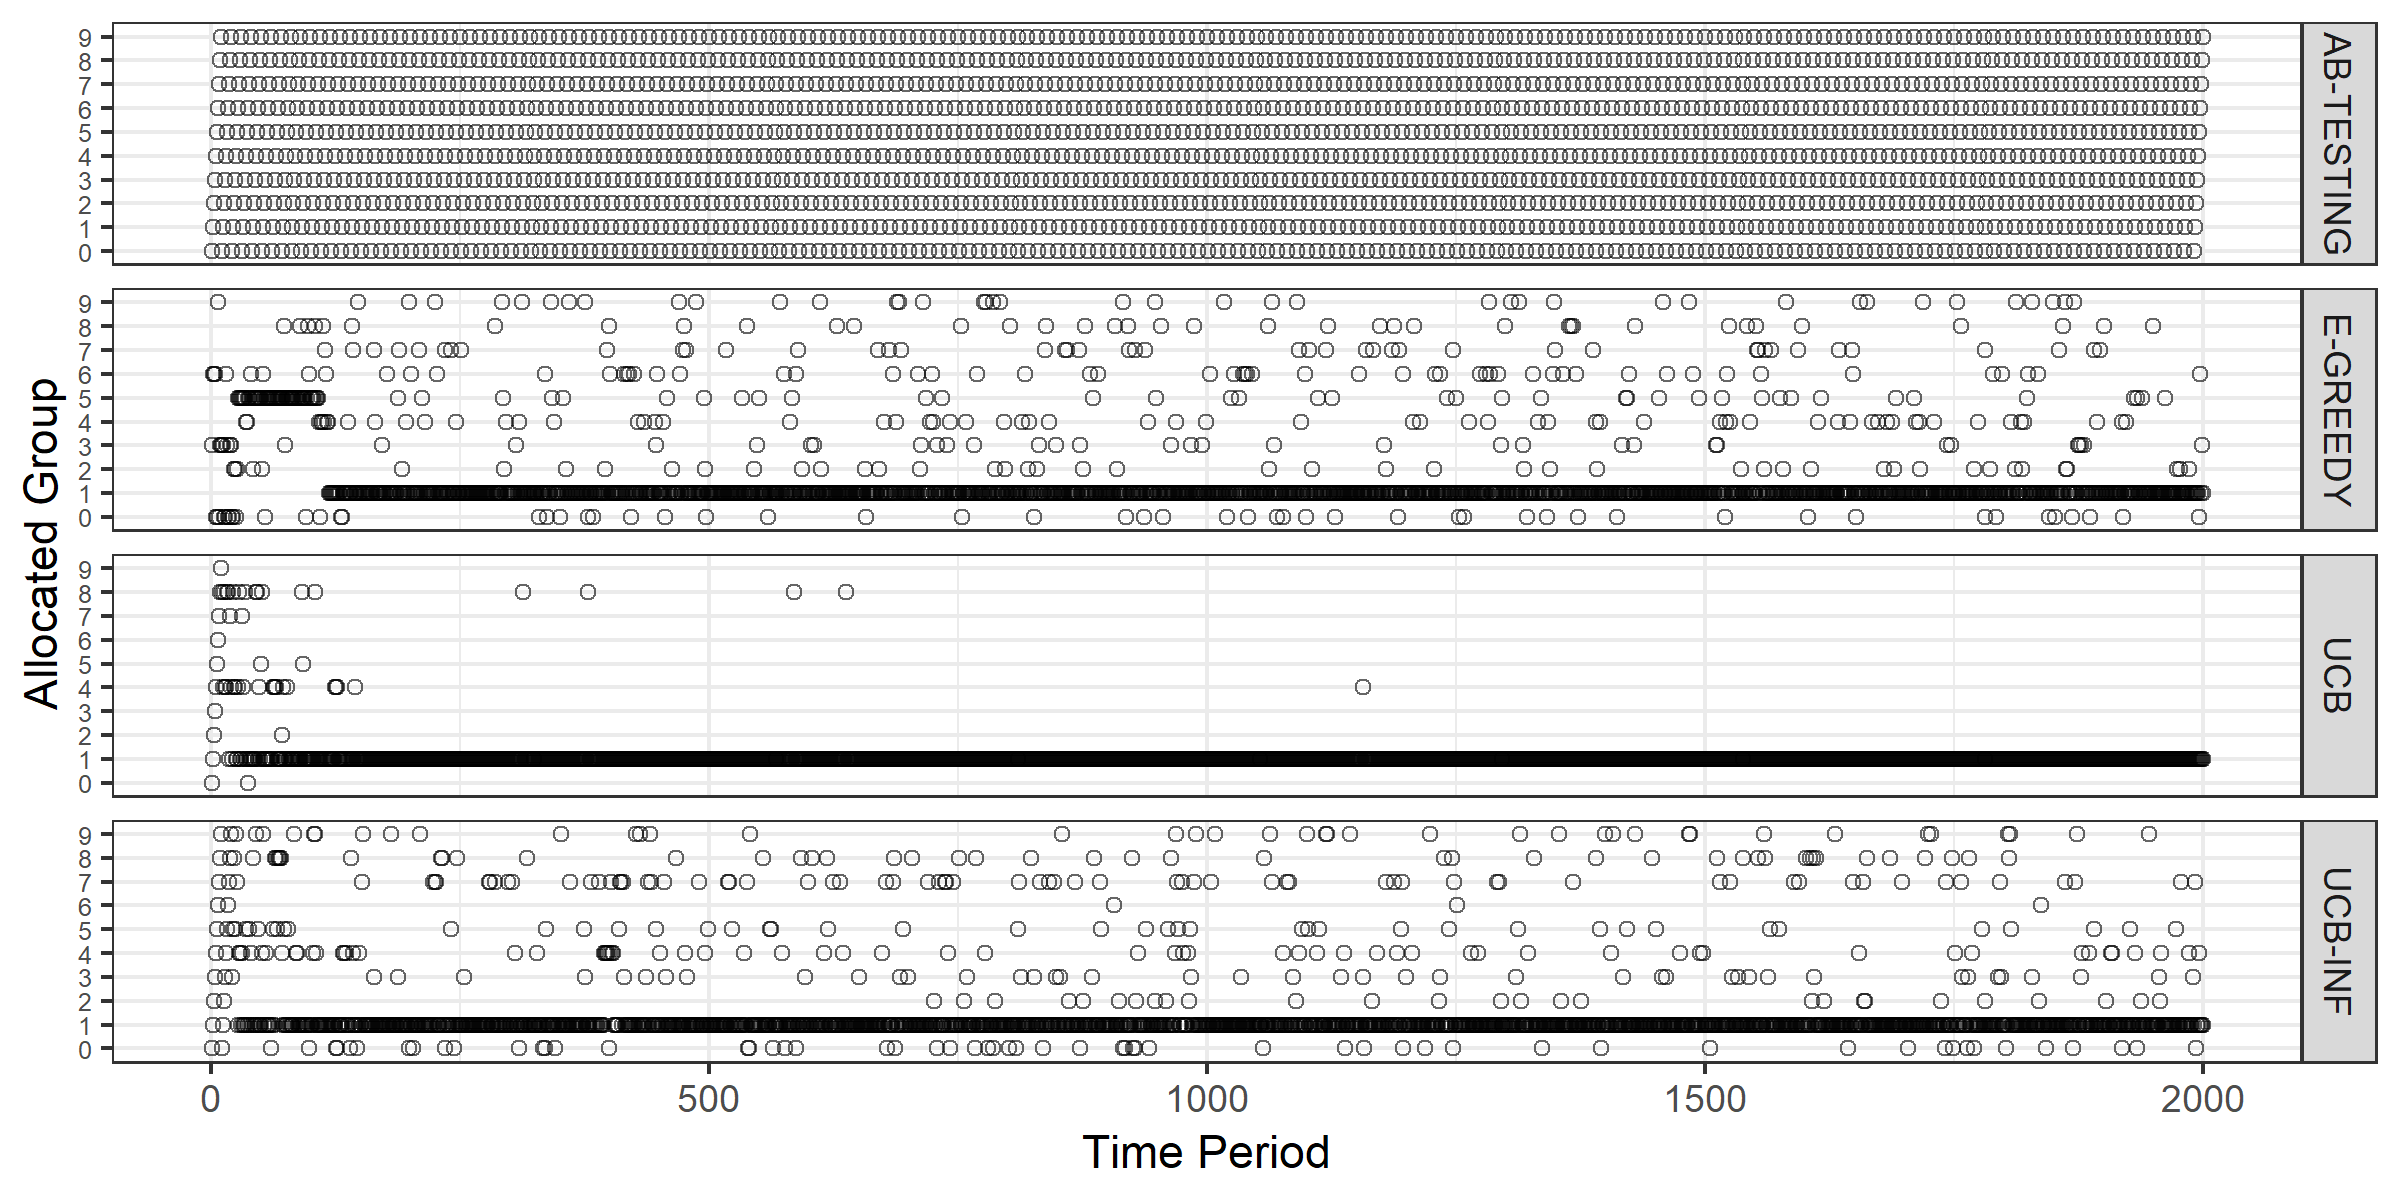
\includegraphics[width=\textwidth]{figs/group.png}
      \caption{This figure shows the allocations of subjects to treatment groups over time for different allocation procedures}
      \label{group}
\end{figure}

\begin{figure}
  \centering
    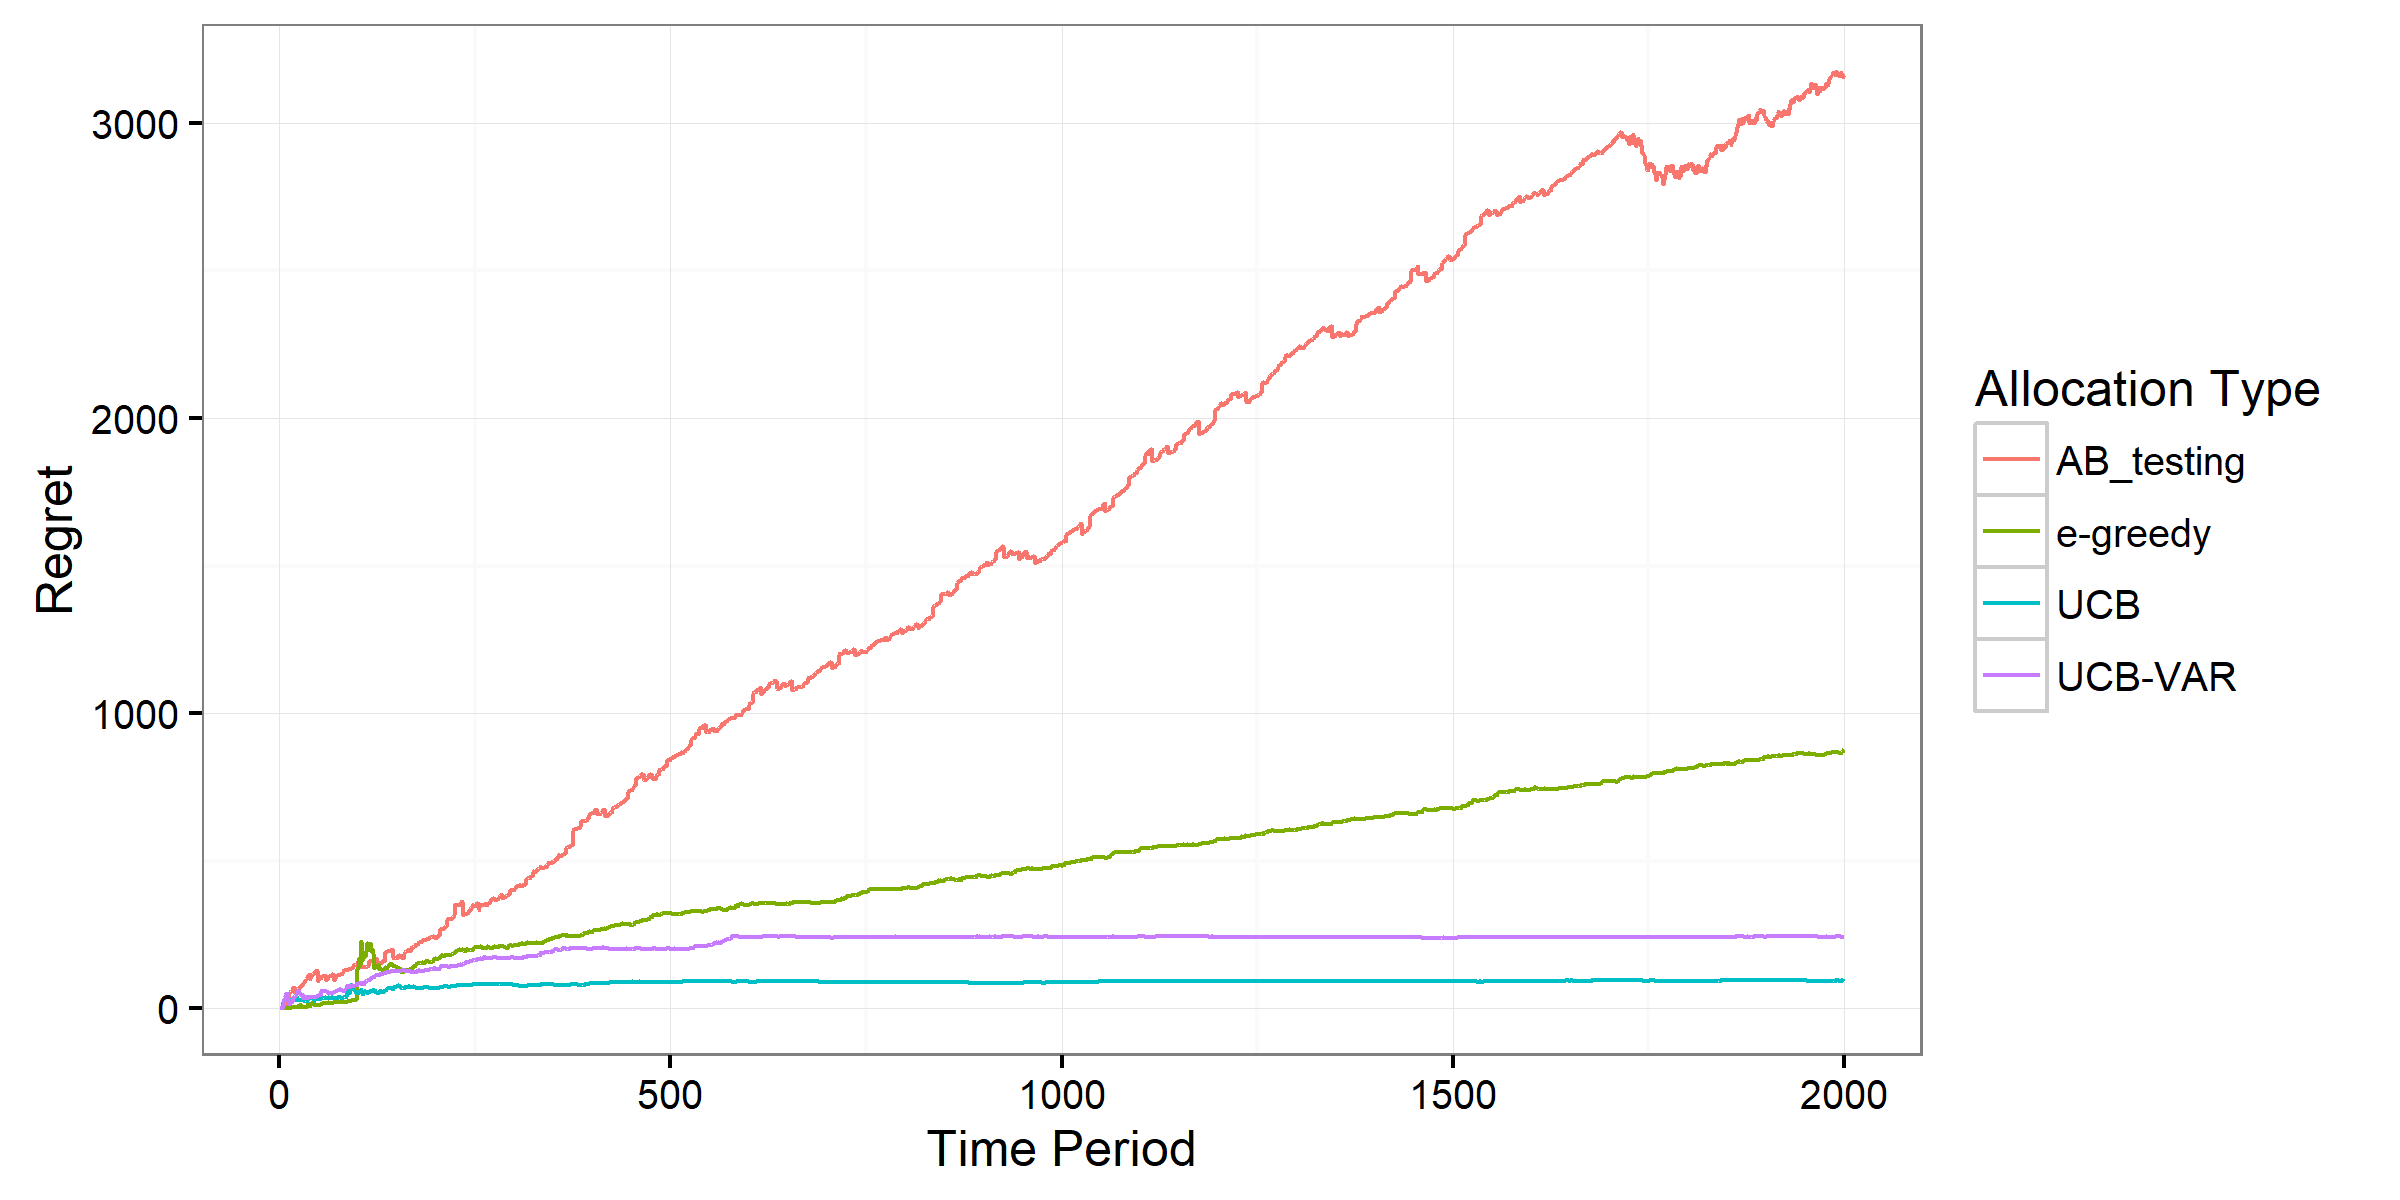
\includegraphics[width=\textwidth]{figs/regret.png}
      \caption{This figure shows the regret of different allocation procedures over time}
      \label{regret}
\end{figure}


\subsection*{Results}

We ran the simulation for A/B testing, UCB, $\epsilon$-greedy and UCB-VAR by allocating subjects to different treatment conditions as per algorithmic suggestions and drawing a value from the outcome distribution of allocated intervention. Fig:\ref{group} shows how subjects are allocated to different interventions by different algorithms. It can be seen that all groups in A/B testing are sequentially allocated until the smallest effect is detected with sufficient power. Once the exploration is done, the rest of the subjects are allocated to group 5 as it has the highest mean outcome. Allocations in UCB are much more efficient and they swiftly converge to group 5. However, most treatment groups barely receive any allocations. For example, group 0 only has two subjects allocated and group 3 only has one subject allocated.  Owing to this, the estimation of mean and variance is inaccurate. This can be seen from Fig:\ref{var_rmse} where UCB has the highest RMSE of variance estimation and does not reduce even after all subjects are allocated. This is because the primary objective of UCB is to reduce regret and has one of the best finite time regret bounds among MAB algorithms. Fig:\ref{var} shows the variance estimate provided by different allocation procedures at different time periods. The black solid line represents the true variances drawn from the uniform distribution of 0 and 5. 


Both $\epsilon$-greedy and UCB-VAR converge to the best intervention, however, exploration in $\epsilon$-greedy is random while exploration in UCB-VAR is selective. In UCB-VAR, allocations are made to those interventions where there is high uncertainty in the variance estimate. Also, the variance change tolerance parameter helps in further reducing the regret. Once there is certainty in the variance estimate, UCB-VAR switches to UCB more frequently. This can be seen in Fig:\ref{regret} where after initial exploration, the regret line of UCB and UCB-VAR stay parallel. In contrast, the regret line of $\epsilon$-greedy keeps increasing as more allocations are made. The variance estimation properties of A/B testing, UCB-VAR and $\epsilon$-greedy are equally good because of continuous exploration across all arms by A/B testing and $\epsilon$-greedy and selective exploration by UCB-VAR. Fig:\ref{var} shows that, for all arms, the estimate of the variance converges to true variance for every algorithm except UCB. This shows that the variance estimation properties of UCB-VAR are as good as A/B testing.

Overall, we see that UCB-VAR does sacrifice the overall utility but the regret is still comparable to that of UCB which has one of the best regret bounds among MAB algorithms. At the same time, the variance estimation of UCB-VAR is as good as A/B testing. 



\begin{figure}
  \centering
    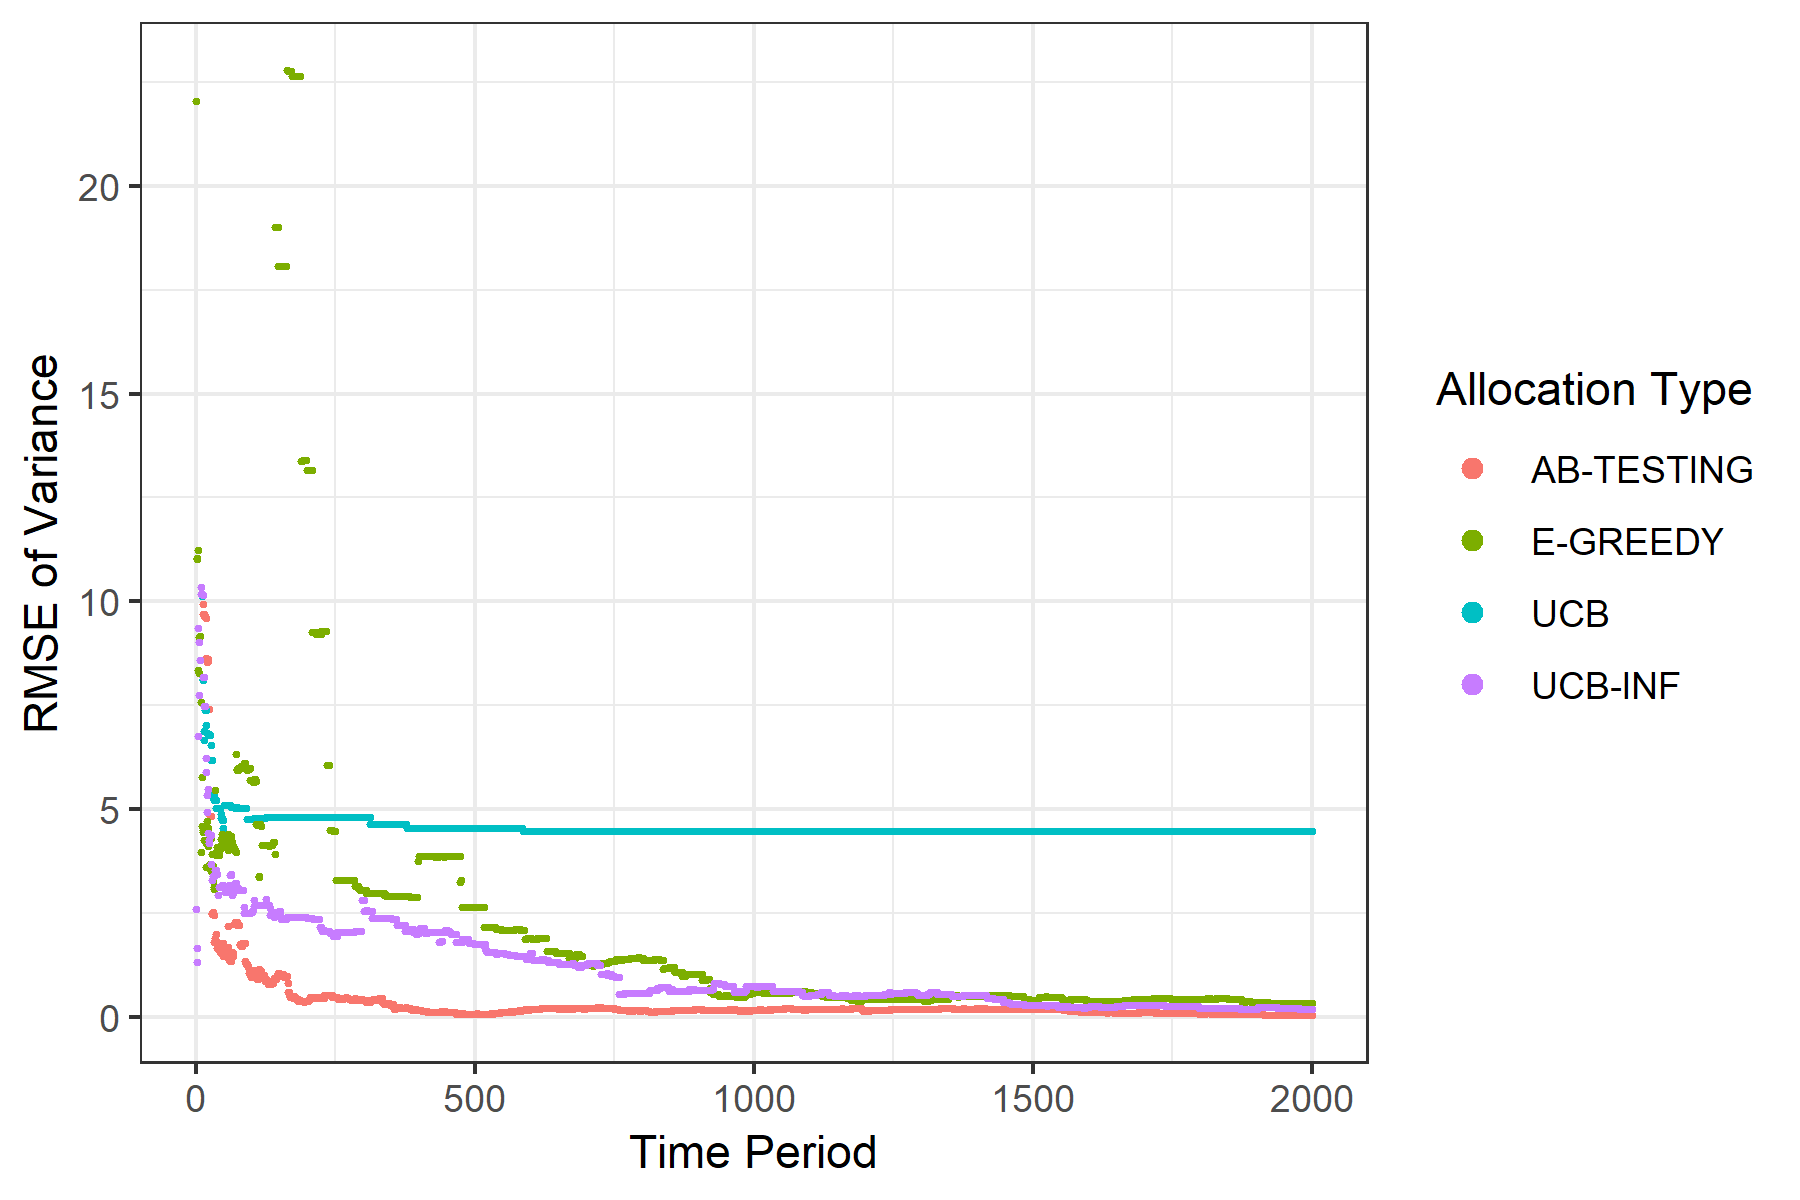
\includegraphics[width=\textwidth]{figs/var_rmse.png}
      \caption{This figure shows the root mean squared error of variance estimation by different allocation procedures over time}
      \label{var_rmse}
\end{figure}


\begin{figure}[]
  \centering
    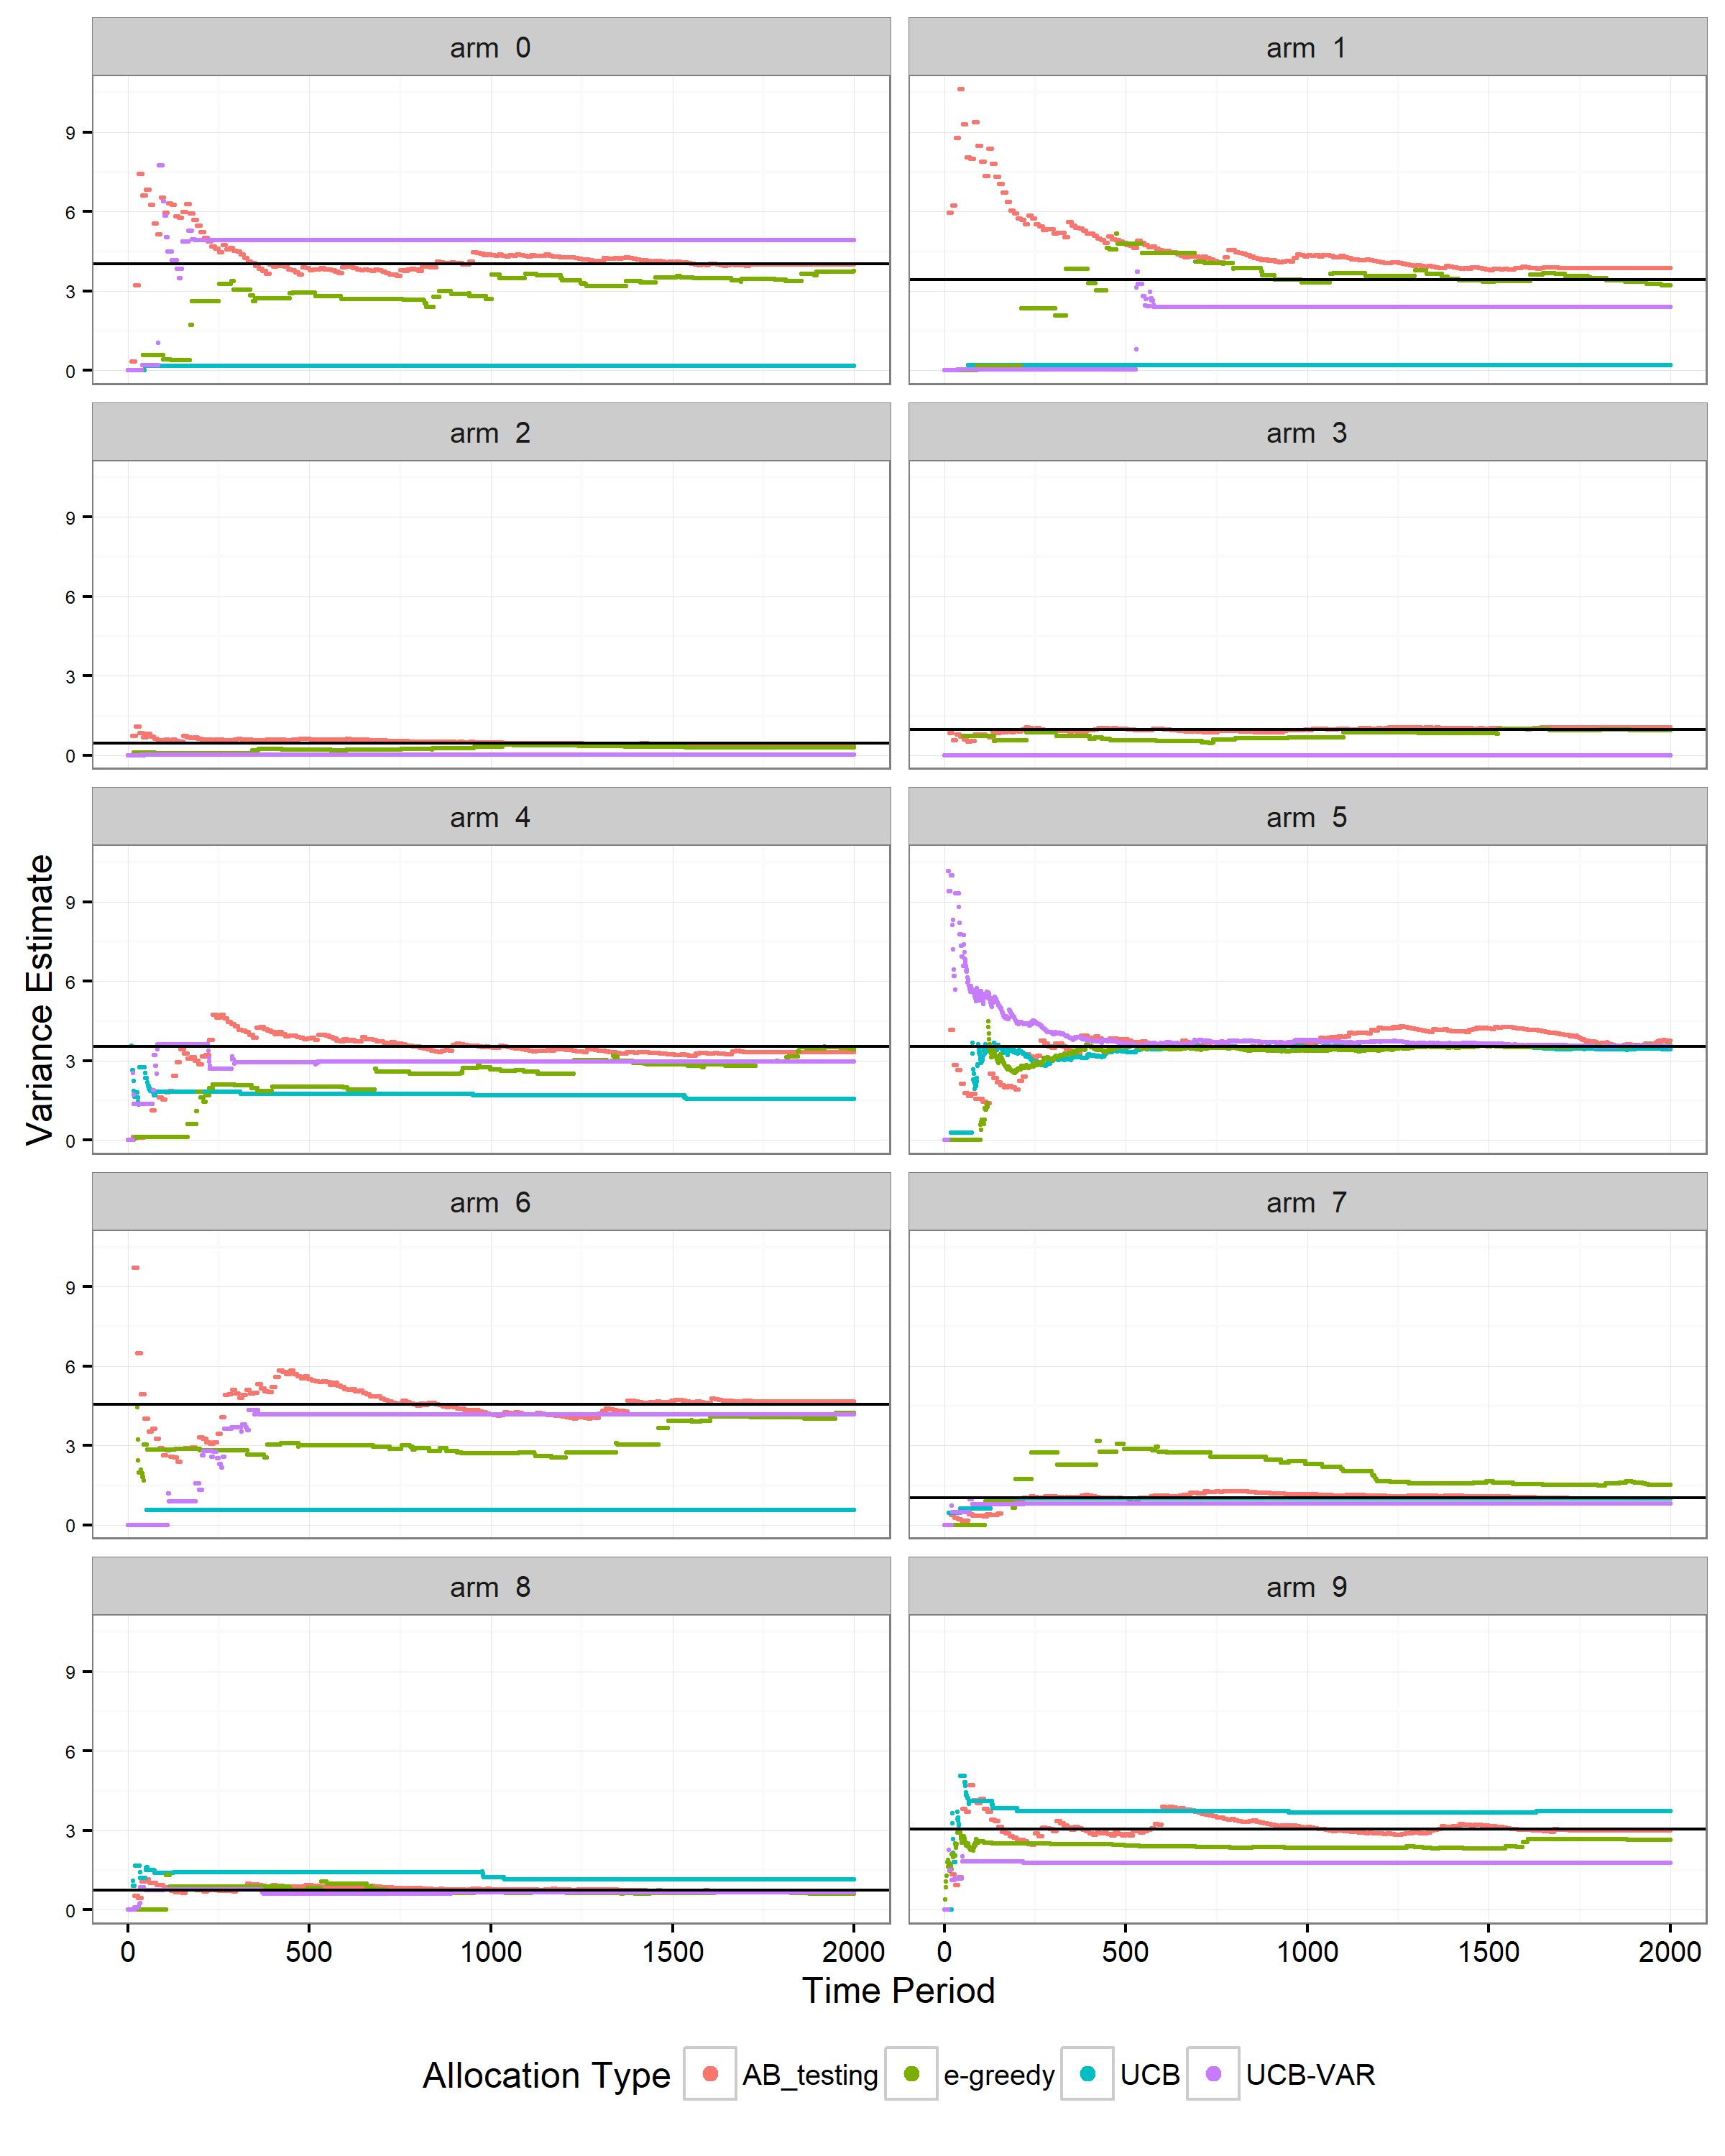
\includegraphics[width=\textwidth]{figs/var.png}
      \caption{This figure shows the variance estimate of different algorithms for multiple interventions}
      \label{var}
\end{figure}




\section*{Conclusion and Future Work}

In this paper, we present a new MAB algorithm called UCB-VAR, where the objective of the allocation procedure is not only to minimize regret but also to estimate the mean and variance of outcome distributions accurately. We conducted simulations and compared the performance of UCB-VAR with A/B testing and other MAB algorithms like UCB and $\epsilon$-greedy. We show that UCB-VAR has regret comparable to that of UCB algorithm while estimation of mean and variance of outcome distributions is comparable to that of A/B testing. This algorithm is very useful in multiple domains like online experimentation, marketing, clinical trials, and public policy. It is especially effective in scenarios where there are a limited number of subjects available for allocation and the utility maximization is as important as estimating outcome distributions accurately. 

In future, we want to use an algorithm similar to UCB-VAR and investigate how the allocations change by optimizing for treatment effect distributions instead of outcome distribution. We also want to derive the asymptotic and finite time regret and variance bounds using statistical theory for UCB-VAR.

\newpage

\bibliography{references}

\begin{comment}
\begin{figure}
  \centering
    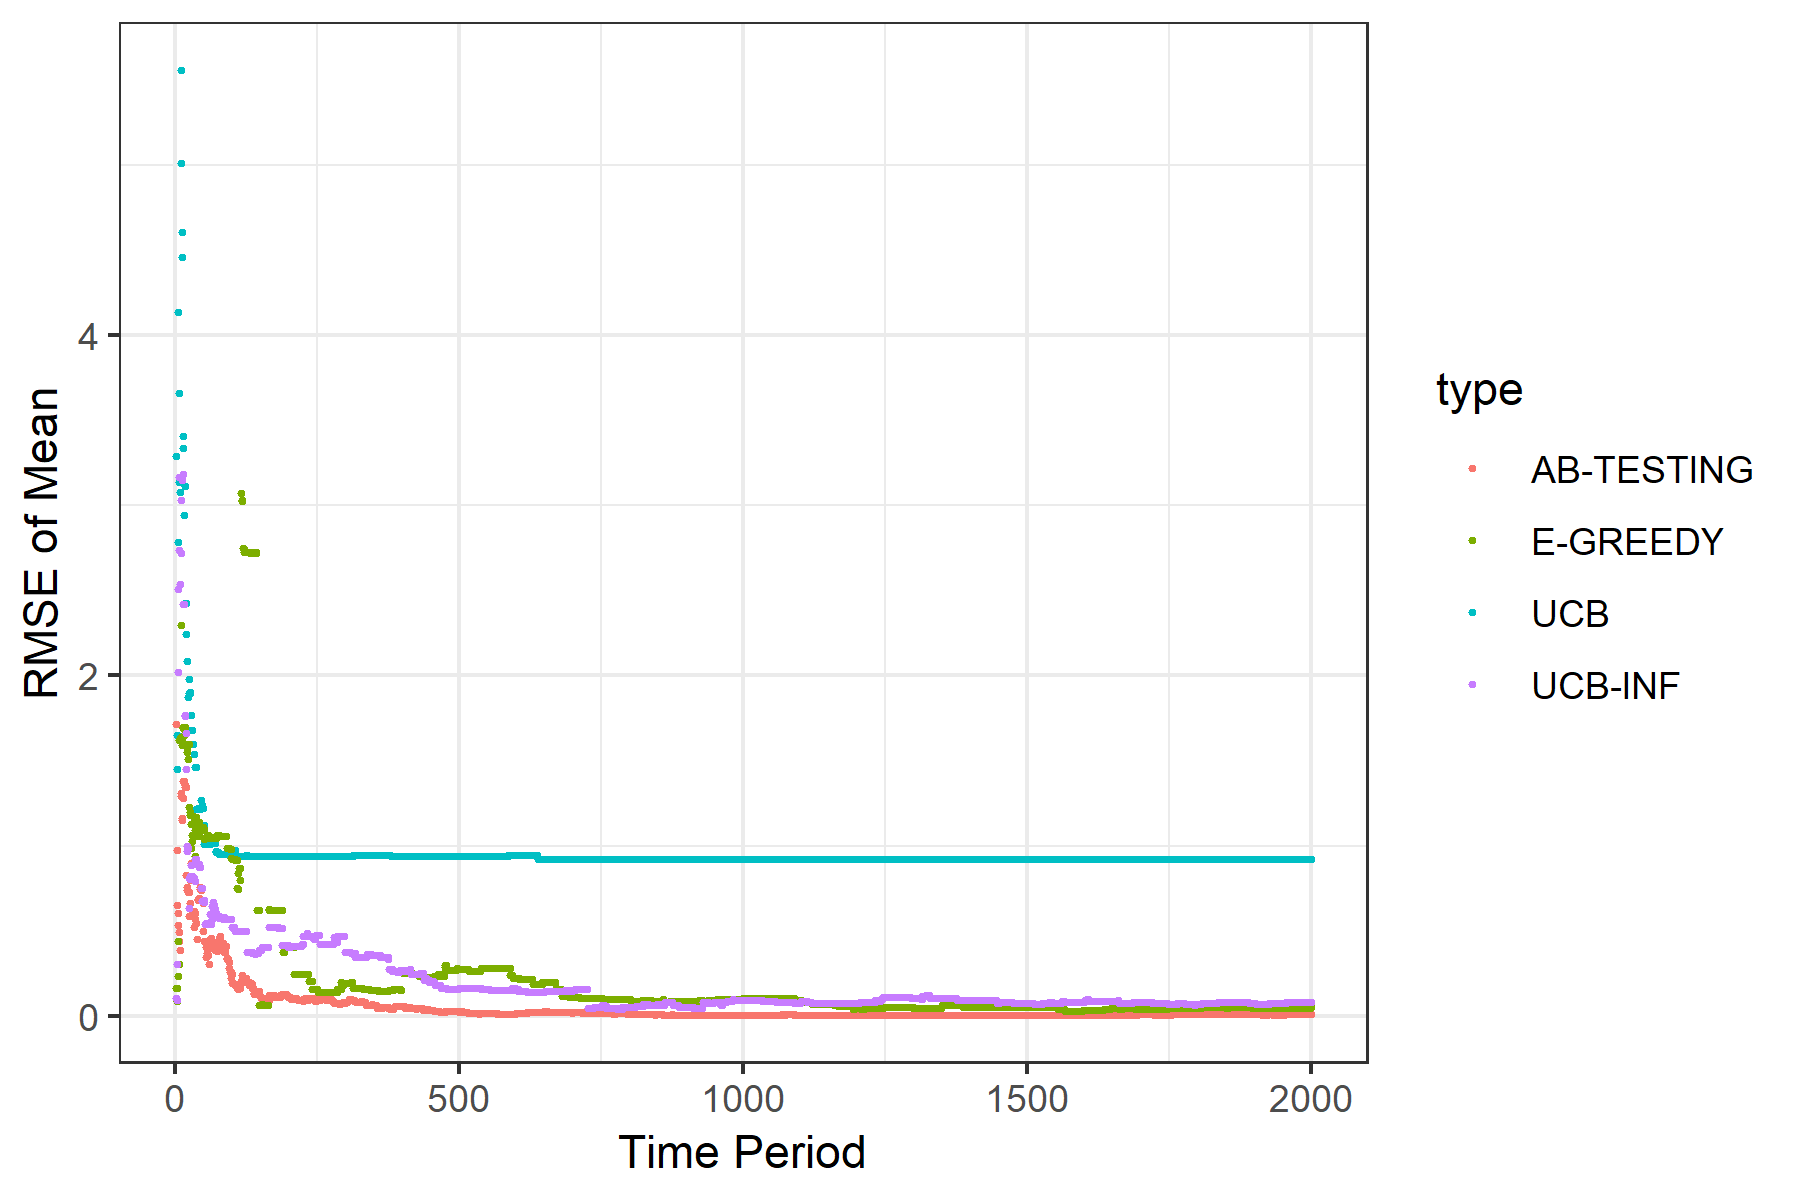
\includegraphics[width=\textwidth]{figs/mean_rmse.png}
      \caption{This figure shows the root mean squared error of variance estimation by different allocation procedures over time}
    \label{mean_rmse}
\end{figure}

\end{comment}


\end{document}


